\subsection{B-spline as activation functions}\label{sec:Bsplines}
In this section, we consider the power of ReLU as activation functions
\begin{equation}
  \label{relup}
{\rm ReLU}^k(x)=[x_+]^k. 
\end{equation} 


We consider the following neuron network function class 
with one hidden layer:
\begin{equation}
\label{VkN}
V_N^k=\left\{\sum_{i=1}^Na_i(w_i\cdot x+b_i)_+^k, a_i, b_i\in\mathbb R^1, w_i\in \mathbb R^{1\times d}\right\}.
\end{equation}
We note that $V_N^k$ is not a linear vector space.  The definition of
neural network function class such as \eqref{VkN} can be traced back
in \cite{mcculloch1943logical} and its early mathematical analysis can be found in \cite{hornik1989multilayer,cybenko1989approximation,funahashi1989approximate}.

The functions in $V^k_N$ as defined in \eqref{VkN} will be known as finite neuron functions in this paper.
\begin{lemma}
  For any $k\ge 1$, $V_N^k$ consists of functions that are piecewise
  polynomials of degree $k$ with respect to a grid whose boundaries are
  given by intersection of the following hyperplanes
$$
w_ix + b_i=0,\quad 1\le i\le N.
$$
see Fig \ref{fig:1} and Fig \ref{fig:3}. Furthermore, if $k\ge m$,
$$
V_N^k(\Omega)\subset H^k(\Omega)\subset H^m(\Omega),
$$
where $\Omega$ is a bounded domain in $\mathbb{R}^d$.
\end{lemma}
\begin{figure}[!ht]
\begin{center}
%$(10, 10)$ $(20, 20)$ $ (40,40)$ 
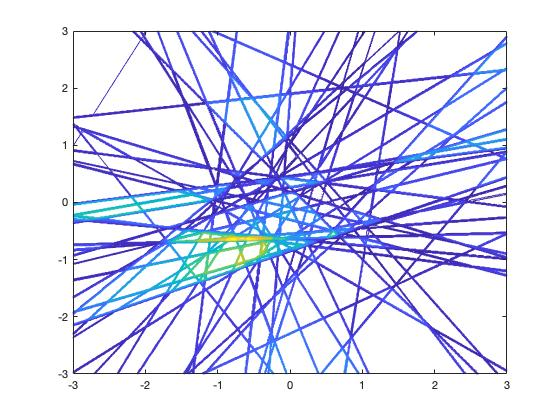
\includegraphics[width=.3\textwidth]{6dl/figures/dnn1-50.jpg}    
\end{center}
\caption{Hyperplanes with $\ell=1$, where $\ell$ is the depth of the neural network in \eqref{NNL}.}
\label{fig:1}
\end{figure} 		
 

The main goal of this section is to prove that the 
following type of error estimate holds, for some $\delta\ge 0$,
\begin{equation}\label{VNerror}
\inf_{v_N\in V_N^k}\|u- v_N \|_{H^m(\Omega)} \lesssim 
N^{-{1\over 2}-\delta}.
\end{equation} 
We will use two different approaches to establish \eqref{VNerror}.
The first approach, presented in \S\ref{sec:Bsplines}, mainly follows
\cite{hornik1994degree} and \cite{siegel2020approximations} that gives
error estimates for a general class of activation functions.  The
second approach follows
\cite{klusowski2016uniform} that gives error estimates specifically
for ReLU activation function.

We assume that $\Omega\subset\mathbb R^d$ is a given bounded domain.
Thus,
\begin{equation}
  \label{T}
T=\max_{x\in \bar{\Omega}} \|x\|<\infty.  
\end{equation}
The activation function ${\rm [ ReLU]}^k$ \eqref{relup} is related to
cardinal B-Splines.  A cardinal B-Spline of degree $k\ge 0$
denoted by $b^k$, is defined by convolution as
\begin{equation}
	b^k(x)=(b^{k-1}*b^0)(x)=\int_\mathbb{R}b^{k-1}(x-t)b^0(t)dt,
\end{equation}
where 
\begin{equation}
b^0(x)=\left\{
		     \begin{array}{lr}
		    1 & x\in[0,1),\\
		    0 & \hbox{otherwise}.
		     \end{array}
	\right.
\end{equation}
\begin{figure}
\begin{center}
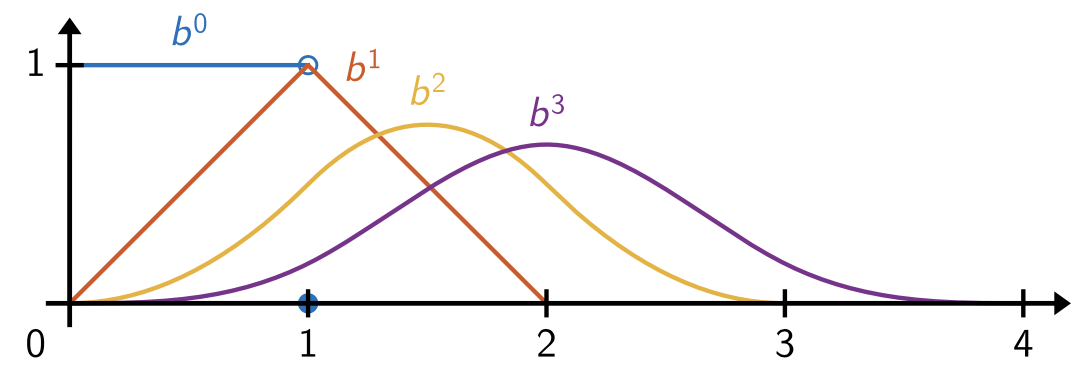
\includegraphics[width=0.5\textwidth]{6DL/figures/B-spline.png}   
\caption{Plots of some B-spline basis}
\label{bk}
\end{center}
\end{figure}
More explicitly, see \cite{de1971subroutine}, for any
$x\in[0,k+1]$ and $k\geq 1$, we have 
	\begin{equation}
	b^k(x)=\frac{x}{k}b^{k-1}(x)+\frac{k+1-x}{k}b^{k-1}(x-1),
	\end{equation}
or
	\begin{equation}\label{splinetorelu}
	b^k(x)=(k+1)\sum_{i=0}^{k+1} w_i(i-x)_+^k \hbox{~and~} w_i={\displaystyle\prod_{j=0,j\neq i}^{k+1}} \frac{1}{i-j}.
	\end{equation}
We note that all $b^k$ are locally supported and see Fig.~\ref{bk} for their plots. 

For an uniform grid with mesh size $h=\frac{1}{n+1}$, we define
	\begin{equation}
	b^k_{j,h}(x)=b^{k}(\frac{x}{h}-j).
	\end{equation}
Then the cardinal B-Spline series of degree $k$ on the uniform grid is 
\begin{equation}\label{Skn}
S_N^k=\Big\{v(x)=\sum_{j=-k}^{N}	c_jb^k_{j,h}(x)\Big\}.
\end{equation}
\begin{lemma} For $V_N^k$ and $S_N^k$ defined by \eqref{VkN} and
  \eqref{Skn}, we have
\begin{equation}
    \label{SV}
S_N^k\subset V_{N+k+1}^k.    
  \end{equation}
As a result, for any bounded domain $\Omega\subset \mathbb R^1$, we have
\begin{equation}
  \label{SVerror}
\inf_{v\in V_{N}^k}\|u-v\|_{m,\Omega} 
\le \inf_{v\in S_{N-k-1}^k}\|u-v\|_{m,\Omega} \lesssim N^{m-(k+1)} \|u\|_{k+1,\Omega}.
\end{equation}
\end{lemma}

\iffalse
Given an activation function $\sigma\in L^1(\mathbb R)$, consider its Fourier transformation:
\begin{equation}
  \label{Fsigma}
\hat \sigma(a) = \frac{1}{2\pi}\int_{\mathbb{R}} \sigma(t)e^{-iat}dt. 
\end{equation}
For any $a\neq 0$ with $\hat \sigma(a)\neq 0$, by making a change of variables 
$t = a^{-1}\omega\cdot x + b$ and $dt = db$, we have
 \begin{equation}
 \begin{aligned}
\hat{\sigma}(a)&=\frac{1}{2\pi}\int_{\mathbb{R}}\sigma(a^{-1}\omega\cdot x+b)e^{-ia( a^{-1}\omega\cdot x+b)}db = e^{-i\omega \cdot x}\frac{1}{2\pi}\int_{\mathbb{R}}\sigma(a^{-1} \omega\cdot x+b)e^{-iab}db.
 \end{aligned}
 \end{equation}
This implies that
\begin{equation}\label{FourierExp}
 e^{i\omega \cdot x} = \frac{1}{2\pi\hat{\sigma}(a)}\int_{\mathbb{R}}\sigma(a^{-1}\omega\cdot x+b)e^{-iab}db.
\end{equation}
We write $ \hat{u}(\omega) = e^{-i\theta(\omega)} | \hat{u}(\omega)|$
and then obtain the following integral represntation:
\begin{equation}\label{integral_representation01}
u(x) = \int_{\mathbb{R}^d} e^{i\omega\cdot x}\hat{u}(\omega)d\omega = 
\int_{\mathbb{R}^d}\int_\mathbb{R}\frac{1}{2\pi\hat{\sigma}(a)}
\sigma\left(a^{-1} \omega\cdot x+b\right)|\hat{u}(\omega)|e^{-i(ab+\theta(\omega))}dbd\omega
\end{equation}
Now we consider activation function $\sigma(x)=b^k(x)$ and $\hat \sigma$ be the
Fourier transform of $\sigma(x)$. Note that, by \eqref{bk}, 
\begin{align}\label{splineFourier}
\hat{\sigma}(a)=\left({1-e^{-ia}\over ia}\right)^{k+1}=\left({2\over a}\sin {a\over 2}\right)^{k+1}e^{-{ia(k+1)\over 2}}.
\end{align}

We first take $a=\pi$ in \eqref{splineFourier}. Thus,
\begin{equation}
  \label{pi1}
\hat\sigma(\pi)=
\left({2\over \pi}\right)^{k+1}e^{-{i\pi (k+1)\over 2}}.
\end{equation}
Combining \eqref{integral_representation01} and \eqref{pi1}, we obtain
that
\begin{equation}
  \label{splinerep0}
u(x) = 
\frac{1}{4}\left({\pi\over 2}\right)^{k}\int_{\mathbb{R}^d}\int_\mathbb{R}
\sigma\left(\pi^{-1}\omega\cdot x+b\right)|\hat{u}(\omega)|e^{-i(\pi b + {\pi (k+1)\over 2}+\theta(\omega))}dbd\omega
\end{equation}
An application of the Monte Carlo method in Lemma \ref{MC} to the integral representation \eqref{splinerep0} leads to the following estimate.
\begin{theorem}\label{splinestratify}
For any $0\le m\le k$, if $u\in {B}^{m+1}(\Omega)$, there exist $\omega_i\in \mathbb{R}^d$, $b_i\in \mathbb{R}$ such that
\begin{equation}
\left \|u - u_{N}\right\|_{H^{m}(\Omega)}\lesssim  N^{-{1\over 2}} \|u\|_{{B}^{m+1}(\Omega)}
\end{equation}
with
\begin{equation}
u_{N}(x)=\sum_{i=1}^{N} \beta_i b^k\left(\pi^{-1} \omega_i\cdot x+b_i\right).
\end{equation} 
\end{theorem}

Based on the integral representation \eqref{splinerep0}, a stratified analysis similar to the one in \cite{siegel2020approximations} leads to the following result.
\begin{theorem}
For any $0\le m\le k$ and positive $\epsilon$,  if $u\in {B}^{m+1+\epsilon}(\Omega)$, , there exist $\omega_i\in \mathbb{R}^d$, $b_i\in \mathbb{R}$ such that
\begin{equation}\label{straunbdd}
\left\|u - u_{N}\right\|_{H^{m}(\Omega)}\le  N^{-{1\over 2}-{\epsilon \over (d+1)(2+\epsilon)}} \|u\|_{{B}^{m+1+\epsilon}(\Omega)}
\end{equation}
with
\begin{equation}
u_{N}(x)=\sum_{i=1}^{N} \beta_i b^k\left(\bar \omega_i\cdot x+b_i\right) .
\end{equation} 
\end{theorem}
Next, we try to improve the estimate \eqref{straunbdd}. Again, we will use \eqref{integral_representation01}. Let $\displaystyle a_\omega=4\pi\lceil {\|\omega\|\over 4\pi}\rceil + \pi$ in \eqref{splineFourier} and $\displaystyle \bar\omega ={\omega\over a_\omega}$. We have
 \begin{equation}
\hat{\sigma}(a_\omega)=\left({2\over a_\omega}\right)^{k+1}, \quad \|\omega\| + \pi\le a_\omega\le \|\omega\|+5\pi,\quad \|\bar\omega\|\le 1,
 \end{equation}
which, together with \eqref{integral_representation01}, indicates that
 \begin{equation}\label{integral_representation}
 \begin{split}
  u(x) =  \int_{\mathbb{R}^d}\int_\mathbb{R}\frac{1}{2\pi}
  \sigma\left(\bar \omega\cdot x+b\right)\left({a_\omega\over 2}\right)^{k+1}\hat{u}(\omega)e^{-ia_\omega(b+{k+1\over 2})}dbd\omega.
\end{split}
 \end{equation}


\begin{theorem}
If $u\in {B}^{k+1}(\Omega)$, there exist $\|\bar \omega_i\|\le 1$, $|b_i|\le T + k+1$ such that
\begin{equation}\label{d+1}
\left\|u - u_{N}\right\|_{H^{m}(\Omega)}\lesssim  N^{-{1\over 2}-{1\over d+1}} \|u\|_{{B}^{k+1}(\Omega)}
\end{equation}
with
\begin{equation}
u_{N}(x)=\sum_{i=1}^{N} \beta_i b^k\left(\bar \omega_i\cdot x+b_i\right) .
\end{equation} 
\end{theorem}
\begin{proof}
We write \eqref{integral_representation} as follows
$$
\displaystyle u(x)= \int_{\mathbb{R}^d}\int_\mathbb{R}
g(x, b, \omega)\rho(b,\omega) dbd\omega
$$
with 
$$ 
\hat{u}(\omega) = e^{-i\theta(\omega)} | \hat{u}(\omega)|,\quad \tilde \theta(\omega)=\theta(\omega) + a_\omega(b+{k+1\over 2})
$$ and 
\begin{equation}\label{eq:g}
g(x, b, \omega) = \sigma\left({\bar \omega}\cdot x+b\right)sgn(\cos \tilde\theta(\omega)),
\end{equation}
\begin{equation}\label{eq:rho}
\rho(b,\omega) = \frac{1}{(2\pi)^d}\left({a_\omega\over 2}\right)^{k+1}| \hat{u}(\omega)||\cos \tilde\theta(\omega)|.
\end{equation} 
Note that
\begin{equation}
\|\bar\omega\|\le 1, \quad |b|\le T+k+1.
\end{equation} 
Let 
$$
G=\{(\omega, b): \omega\in \mathbb{R}^d,\ |b|\le T+k+1\}, \ \tilde G=\{(\bar \omega, b): \|\bar \omega\| \le 1,\ |b|\le T+k+1\}.
$$
For any positive integer $n$, divide $\tilde  G$ into $\tilde  M(\tilde  M\le {n\over 2})$   nonoverlapping subdomains, say 
$\tilde  G=\tilde  G_1\cup \tilde  G_2\cup \cdots \cup\tilde  G_{\tilde M}$, such that
\begin{equation}
|b-b'|\lesssim n^{-{1\over d+1}},\quad |\bar\omega - \bar\omega'|\lesssim  n^{-{1\over d+1}}, \quad (\bar\omega, b),\ (\bar\omega', b')\in \tilde G_i,\ 1\le i\le \tilde M.
\end{equation} 
Define $M=2\tilde  M$ and for $1\le i\le \tilde M$,
$$
G_i = \{(\omega, b): (\bar \omega, b)\in \tilde  G_i, \ \cos \tilde\theta(\omega)\ge 0\},\ 
G_{\tilde  M+i} = \{(\omega, b): (\bar \omega, b)\in \tilde  G_i, \ \cos \tilde\theta(\omega)\le 0\}.
$$
Thus, $G=G_1\cup G_2\cup \cdots \cup G_M$ with $\tilde  G_i\cap \tilde G_j=\varnothing$ if $i\neq j$, and 
\begin{equation}
|b-b'|\lesssim n^{-{1\over d+1}},\quad |\bar\omega - \bar\omega'|\lesssim  n^{-{1\over d+1}}, \quad sgn(\cos \tilde\theta(\omega))=sgn(\cos\tilde \theta(\omega')).
\end{equation} 
Let $n_i=\lceil \lambda(G_i)n\rceil$, $N=\displaystyle \sum_{i=1}^M n_i$ and
\begin{equation}
u_{N}(x)=\|\rho\|_{L^1(G)}\sum_{i=1}^{M} \frac{\lambda(G_{i})}{n_{i}} \sum_{j=1}^{n_{i}}g(x,\theta_{i,j}).
\end{equation}
It holds that
\begin{equation}\label{eq:sum}
\begin{split}
\mathbb{E}\left(\left\|u - u_{N}\right\|_{H^{m}(\Omega)}^{2}\right)\le&
\|\rho\|_{L^1(G)}\sum_{i=1}^{M}  \frac{\lambda^2(G_i)}{n_{i}}  \sup_{\theta_{i},\theta_{i}'\in G_i} \| g(x,\theta_i) - g(x,\theta_i')\|^2_{H^m(\Omega)}
 \end{split}
\end{equation}
with $\theta=(b, \omega)$. 
For any $(b, \omega)\in G_i$, $1\le i\le M$, if $k\ge m+1$,
\begin{equation}
|g(x,\theta) - g(x,\theta')| \lesssim |b-b'| + |\omega - \omega'| \lesssim   n^{-{1\over d+1}}
\end{equation}
Thus,
\begin{equation}
 \sum_{i=1}^{M}  \frac{\lambda^2(G_i)}{n_{i}}  \sup_{\theta_{i},\theta_{i}'\in G_i} \| g(x,\theta_i) - g(x,\theta_i')\|^2_{H^m(\Omega)}  
 \lesssim  n^{-{2\over d+1}} |\Omega|.
\end{equation}
Thus,
\begin{equation}\label{eq:}
\begin{split}
\mathbb{E}\left(\left\|u - u_{N}\right\|_{H^{m}(\Omega)}^{2}\right)\lesssim&   n^{-1-{2\over d+1}} |\Omega|\|\rho\|_{L^1(G)}.
 \end{split}
\end{equation}
Since $a\le \|\omega\|+5\pi$, 
$$
\|\rho\|_{L^1(G)}\lesssim \int_G (\|\omega\| + 1)^{k+1}|\hat u(\omega)|d\omega db \lesssim \|u\|_{B^{k+1}(\Omega)}.
$$
Note that $n\le N\le 2n$. Thus, there exist $\omega_i\in \mathbb{R}^d$, $\beta_i$, $b_i\in \mathbb{R}$ such that
\begin{equation}
\left\|u - u_{N}\right\|_{H^{m}(\Omega)}\lesssim  N^{-{1\over 2}-{1\over d+1}} \|u\|_{B^{k+1}(\Omega)},
\end{equation}
which completes the proof.
\end{proof}

The above analysis can also be applied to more general activation functions with compact support. 
\begin{theorem}
Suppose that $\sigma\in W^{m+1,\infty}(\mathbb{R})$ that has a compact
support. If for any $a>0$, there exists $\tilde a>0$ such that
\begin{equation}
\tilde a\gtrsim a,\quad  |\hat\sigma(\tilde a)|\gtrsim a^{-\ell},
\end{equation}
and  $u\in {B}^{\ell}(\Omega)$, then, there exist $\omega_i\in \mathbb{R}^d$ and $b_i\in \mathbb{R}$ such that
\begin{equation}
\left\|u - u_{N}\right\|_{H^{m}(\Omega)}\lesssim  N^{-{1\over 2}-{1\over d+1}} \|u\|_{B^{\ell}(\Omega)},
\end{equation}
where
\begin{equation}
u_{N}(x)=\sum_{i=1}^{N} \beta_i \sigma\left(\bar \omega_i\cdot x+b_i\right) .
\end{equation} 
\end{theorem}

\fi
